\documentclass[article]{jss}
\usepackage{comment}
\usepackage{graphics}
\usepackage{moreverb}

\usepackage{graphics}

\def\Rfunc#1{\textbf{#1()}}
\def\JSfunc#1{\textsl{#1()}}
\def\SVGEl#1{\texttt{<#1>}}
\def\SVGAt#1{\textbf{#1}}

\author{Duncan Temple Lang\\
    Department of Statistics, \\
    Unversity of California at Davis}

\Address{
Duncan Temple Lang \\
Department of Statistics, \\
371 Kerr Hall, \\
One Shields Avenue, \\
Davis \\
CA 95616 \\
U.S.A.
E-mail: \email{duncan@r-project.org}\\
URL: \url{http://www.stat.ucdavis.edu/~duncan}, \url{http://www.omegahat.org}
}

% Define HTTP early = in the abstract.
% Make the transition for the sentence on forms smoother.
% Expand the collection of actions along with PROPERTY.
% Figures identifying the components of an HTTP request and response.

\title{}
\Plainauthor{Duncan Temple Lang}
\Plaintitle{}

\input{myMacros}


\Abstract{
  Scalable Vector Graphics is an XML-based format for static, dynamic,
  interactive graphics.  In this paper, we describe functions in the R
  package \pkg{SVGAnnotate} for annotating graphical content generated
  in R with tooltips, interactive content, animations and general
  functionality provided by scripting capabilities.  These facilities
  post-process the graphics generated via libcairo in R.  We also
  discuss how the approach can be used with other graphics devices in
  R.
}


\Keywords{Graphics, Scalable Vector Graphics, Animation, Interaction}
\Plainkeywords{Graphics, Scalable Vector Graphics, Animation, Interaction}


\begin{document}

%\begin{abstract}\end{abstract}

Compare this approach with the animation package,
i.e. movies of frames generated by R.
We get interactivity, element animation, GUI components, 
programmability within HTML documents and at the element-level.

JSON for serializing R vectors for use in JavaScript code.

\section{Introduction}
R is well-known for its graphical output, be it based on the
traditional graphics model \cite{grz}, the newer grid \cite{grid} and the
higher-level lattice \cite{lattice}.  These graphics systems provide convenient yet
highly customizable facilities for creating static plots.  However, in
the past few years, there has been a dramatic increase in compelling
graphical displays that provide interaction and animation within
plots.  There are various technologies underlying these displays
including Flash and ActionScript, JavaScript, ``mashups'' with, for example,
Google Maps, Google Earth, and Scalable Vector Graphics (SVG).  
We focus our attention on SVG in this paper; we are also exploring 
several of the alternatives.

SVG is a format that provides facilities for drawing complex graphical
displays.  It is similar to both Portable Document Format (PDF) and
Postscript in that it uses vector graphics.  This uses descriptions of
shapes rather than intensities at particular pixels when the graphics
is first created.  This allows the displays to be scaled without
``pixelation'' caused by extrapolating pixel values and allows
abstraction at the level of graphical objects (e.g. circles, squares,
lines, text) rather than pixels.

Since SVG is an XML-based format, it is relatively easy to create and
manipulate SVG displays. The broad collection of XML tools in all
widely-used languages allows us to programmatically post-process SVG
displays generated in any application.  The focus of this paper is how
we can use R's graphical capabilities to create rich static
statistical displays and then post-process them, with access to the
underlying, to embellish them with additional interactive, dynamic
capabilities.

SVG can be displayed via stand-alone applications such as batik and
also within Web browsers.  SVG files can be displayed as separate
pages within a Web browser, and also embedded as an element within a
regular Web page.  As an embedded component, user interactions within
the Web page can update the SVG display, and similarly gestures within
the SVG display can dynamically change the content of the overall
page.

The \pkg{SVGAnnotation} package provides facilities in R to
post-process an SVG document created via R's graphics facilities using
the libcairo-based graphics device. (This is enabled in versions of R
that are compiled with suitable support.)  The package provides
high-level facilities for adding hyperlinks to elements of a plot;
associating popup tooltips with elements of a plot such as points in a
scatterplot or polygons in a map; linking observations across plots;
animating points based on time.  We have also been able to provide
simple-minded graphical user interfaces (GUIs) for exploring
statistical displays and methods using SVG-based R graphics.  The
package also provides lower-level facilities for identifying elements
of the SVG document that correspond to particular elements of
non-standard plots.  These assist other developers in providing
high-level functions for manipulating additional classes of plots in
R.

An important aspect of the philosophy of the \pkg{SVGAnnotation}
package is that one can combine the creation of the plot using regular
R graphics commands, and then programmatically modify and annotate the
resulting SVG document with access to the original data within R.  The
fundamental facilities of the \pkg{SVGAnnotation} package help to
identify the nodes in the SVG document that correspond to elements of
the display. Given these nodes, we can modify them and create a new
SVG document.

These SVG documents can be displayed in stand-alone viewers such as
Batik \cite{batik} or compliant Web browsers such as Opera
\cite{opera} and Firefox \cite{firefox}. They can also be embedded
within HTML documents. The displays can be manipulated by JavaScript
code and the interactivity within the SVG displays can also
programmatically modify the contents of the HTML document and other
SVG displays. This allows the displays to act as semi-live R graphics
devices, with rich interaction and minimal R computations.  If R were
a browser plugin language (e.g. SNetscape \cite{SNetscape}),
interesting interactivity would be feasbile within the context of an
HTML page.


In section 2, we present and discuss several different examples of 
using SVG facilities to provide interaction.
In section 3, we discuss animation of R graphics using SVG.
We then detail the low-level functions provided by the
\pkg{SVGAnnotation} package and 
After this, 

\section{Basics of SVG}


\section{Examples of Annotating SVG within R}

\subsection{ToolTips}
Because the circles are actually paths drawing
the perimeter, tooltips are only displayed
when the mouse is over the perimeter and
not within the interior.
We can draw a filed disc with the background

The tooltips

\subsection{Hyperlinks}
In addition to adding tooltips to elements of a plot or a display that
display when the viewer hovers over the element, we can also allow the
user to click on an element and display a related Web page.  The
function \Rfunc{addAxesLinks} associates hyperlinks with any or all of
the labels on the horizontal and vertical axes and the plot title.
The function endeavors to find the SVG elements corresponding to these
text annotations. It then adds a transparent rectangle ``underneath''
the text, computing the dimensions  of the rectangle from the extent
of the ``letters''.  It then adds a hyperlink element
(a) as the parent of the rectangle and provides the target URL
as the value of the  xlink:href attribute. 

The same mechanism can be used to place a hyperlink on any element
such as a point in the plotting region of a plot or the line of an
axis.  Having identified the XML node which is to have a hyperlink,
one passes this to the function \Rfunc{addLink} along with the target
URL.


\subsection{Linked plots}
SVG allows us to associate actions with different events such as mouse
entering or leaving an element, clicking on an element and so on.  SVG
also allows us to programmatically change the value of an attribute of
an element such as color, whether it is visible or hidden, or even its
location or size. We can combine these two facilities to
allow the user to move over a point in one plot
and have the color of one or more points in other related plots
change.  This gives us linked plots.

To create a linking across points in a plot, we first create the
plots. This can be as simple as a call to the \Rfunc{pairs} function
to create a draftsman's display of the pairwise-scatterplots.
Alternatively, one can create the plots with individual R commands and
arrange them in arbitrary layouts.  As with all graphics discussed in
this paper, we use an SVG graphics device when creating the displays
and then we read the resulting document back into R as an XML tree.
We can then pass this document to the function \Rfunc{linkPlots}
which modifies the document to add support for point-wise linking.

The \Rfunc{linkPlots} function adds a unique identifier attribute to
each SVG element representing a point in each plot in the display. The
identifiers are of the form \verb+plot-i-j+ where i is the plot index
and j is the observation/point index, both starting at 1.  The
function also adds \SVGAt{onmouseover} and \SVGAt{onmouseout} attributes to each of
these point elements in the SVG document.  Each of these are calls to
ECMAScript functions that set the corresponding points in the other
plots and reset the color back to their original values when the mouse
moves away from the point.  
These functions are very simple as they are called with argumens
giving the number of plots in the display and the index of the point
in each to set or unset.  The original color is available to the
\JSFunc{reset_color} as it is stored in an additional attribute in
each SVG element under the name \SVGAt{originalFill}.

The \Rfunc{linkPlots} function also adds the ECMAScript code that
implement these two functions to the document, either as a reference
to the file or by inserting the contents directly.

\begin{figure}
  \centering
  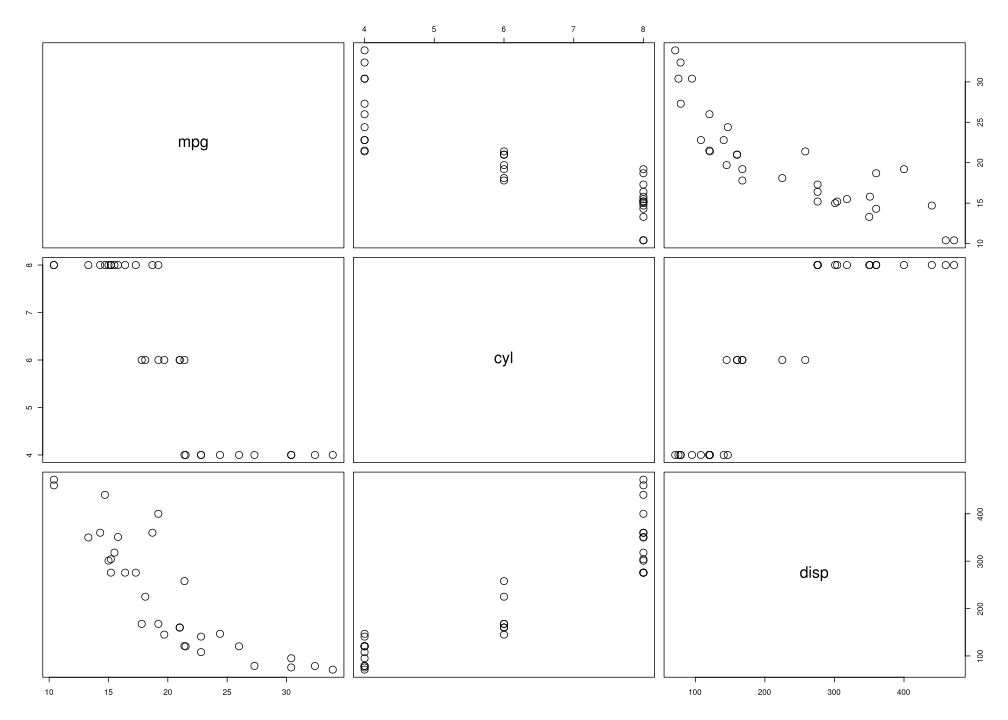
\includegraphics{pairs_link.jpg}
  \caption{Linked plots.  As the viewer moves the mouse over a point,
   the point turns red and so do the corresponding observations in the
   other plots within the display.}
  \label{fig:linkedPairs}
\end{figure}


\subsection{Maps}

\subsection{Non-standard Graphics}
\subsubsection{Ternary Plots}

\subsubsection{Maps}
We can use the \pkg{maps} package in R to draw a map of the US at the
state or county level and color the regions based on the proportion
who voted for Obama.  This gives us the so-called ``purple'' map of
the country.  It is also informative to put tooltips on the different
regions that give the raw counts for the two main candidates and tells
us the percentage voting for Obama.  If we display the map at the
level of states rather than counties, we might also want to allow the
viewer to click on a state and display a table of county-level results 
for that state.
See ../../tests/election.R



A map of the US presidential election results

Cartogram.  We can use the Rcartogram package to create a cartogram
view of the election results to account for different population
densities.  Then we can put tool tips over this to identify the
counties and the proportions.


\subsubsection{graphviz}
Graph layout of nodes and edges is increasingly common but also very
challenging.  The integration of a specialized graph layout engine -
graphviz \cite{graphviz} - with R's graphics systems via
\pkg{Rgraphviz} gives us powerful facilities for creating interesting
data-based graphs.  By post-processing the resulting SVG, we can
provide various forms of interaction and animation.

See Wolfgang Huber's HTML-based graphviz display.

\subsubsection{ggplot2}

\subsubsection{Boxplot}

\section{Animation}

The \Rfunc{animate} function

We have collected the giving the counts for each presidential
candidate in all the elections from 1900 to 2008 for each state. (See
Classes/DataTopics/ElectionHistory.)  For each election, we use the
proportion of the votes to get a shade of ``purple'' and use that to
color each state.  We can animate these over time to visualize how the
states have changed.

There are several ways to implement this animation.  One approach is
to setup 28 animations for each state.  Each animation would set the
new color and wait for a period of time before ending.  We use the SVG
\SVGEl{animate} element for this.

Another approach is to use an ECMAScript function to modify the color
of each state at regular intervals.  We use the SVG element
\SVGEl{setInterval} to do this along with ECMAScript functions that
determine with which election we are currently dealing and to set the
fill value of the style attribute.

We might like to provide the sequence of the $28$ colors for each
state and ask SVG to progress through these at regular intervals.
Unfortunately, this is not a feature of SVG.
See keyTimes and  values.


[Perhaps] In the next section, we illustrate how we can provide a slider
to allow the viewer control which year they see.



\section{GUIs}
The SVG ... library provides interesting
graphical user interface components that can be 
integrated with SVG graphics to make plots
interactive.
We illustrate how these can be used to 
allow viewers control aspects of the display.

\subsection{Time Series}
In this example, we will create a display that plots the exchange rate
against the Euro for several currencies.

\begin{figure}
  \centering
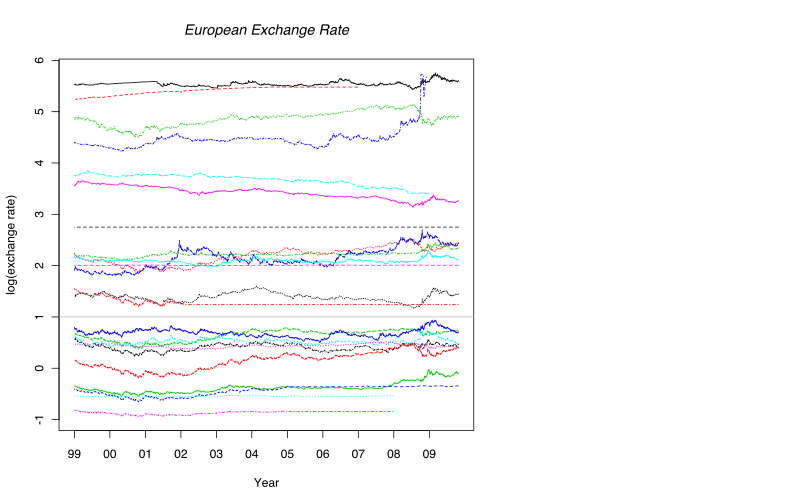
\includegraphics{euSeries.jpg}  
  \caption{Time series of exchange rates against the Euro for 24
    different currencies.  The checkboxes to the right of the plot
    are interactive and allow the viewer to toggle the display of the
    corresponding currency's time series within the plot.}
  \label{fig:euCheckbox}
\end{figure}

We use the carto.net SVG GUI library
to create the checkboxes.
Each interactive checkbox is created 
in ECMAScript code.


We would like to arrange for the plot to redraw
when a time series is added or  removed, e.g.
recalculating the effective limits of the vertical axis.
This is technically feasible within SVG, but rather involved.
It is easier within Flash/ActionScript.  But then we could 
not make use of the R graphics facilities to create the plot.
We are considering implementing a Flash-based graphics device
for R so as to combine the two systems and allow for post-processing
of Flash-based graphics to add animation, etc.


We can also do this across panels of a plot.  For example, we might
draw the time series for the different currencies for each year in a
separate panel by conditioning on year.  Then toggling the currency
would toggle the corresponding curves in each of the panels.
A similar approach




It is of course even simpler to apply this idea to toggle the display
of points on a plot that correspond to different subgroups.  For
example, in the ternary plot example above, we might provide
checkboxes for each of the different baseball positions.

\subsection{Sliders}
In this example, we use a simple-minded approach to providing direct
manipulation interactivity to an R plot.  The end result is a plot
displaying the density of a Beta random variable, along with two
sliders under the plot.  The viewer changes moves the slider thumb to
update the display to show the density corresponding to the updated
value of the parameter.

The natural way to implement this in a regular GUI is to respond to
changes in each slider's position by recalculating and displaying the
density.  Of course, the R functionality to do this is not available
within the SVG viewer at viewing time.  An alternative approach is to
precompute the density curve for all possible combinations of parameters of interest.
We display only one curve at any particular time, using the the
visible attribute on the SVG path corresponding to the density curve
to control whether it is shown or not.  In response to a slider
event, we determine which curve is currently being displayed and which
is to be displayed and toggle their visible attribute.

To create this display,  we plot all of the densities on the same plot, taking
care to specify the appropriate limits for the horizontal and vertical
axes so all parts of each curve are visible.  We use R's regular
graphics functions to create this plot.

\begin{verbatim}
alpha = seq(.01, by = 0.05, length = 30)
beta = seq(.01, by = 0.05, length = 30)

grid = expand.grid(alpha, beta)

f = 'beta.svg'
svg(f)
plot(0, type = "n", xlim = c(0, 1), ylim = c(0, 1.5), xlab = "X", ylab = "density",
         main = "Density of beta distribution")
apply(grid, 1, function(p) curve(dbeta(x, p[1], p[2]), 0, 1, n = 300, add = TRUE))
dev.off()
\end{verbatim}

The next step is to post-process the resulting SVG document.
We read the document into R and find the single plot region.
\begin{verbatim}
doc = xmlParse(f)
box = getViewBox(doc)
p = getPlotRegionNodes(doc)[[1]]
\end{verbatim}
The nodes in the plot region correspond to the curves and in the order
they were originally drawn in R.  So we loop over these and make each
of them hidden and also give each a unique identifier which will allow
us to refer to an individual curve directly within the code to handle
the slider events.  We end this step by making the first curve
visible. 
All of this is done with the folowing R code:
\begin{verbatim}
grid = expand.grid(seq(along = alpha), seq(along = beta))
ids = paste("curve", grid[,1], grid[,2], sep = "-")
invisible(
          sapply(seq(along = ids),
                 function(i)
                     addAttributes(p[[i]], .attrs = c(id = ids[i], visibility = "hidden"))))

addAttributes(p[[1]], .attrs = c(visibility = "visible"))
\end{verbatim}

There are two steps remaining: a) add the two sliders to the display,
b) arrange for the slider events to toggle the curves displayed in the plot.
Step a) involves making space for the two sliders below the plot
and also a text element in which we will display the current values
of the parameters.
In accordance with the SVG GUI library, we create a group for each
slider and give them each a unique name. The sliders will be added to
this group via ECMAScript code.
\begin{verbatim}
svg = xmlRoot(doc)

enlargeSVGViewBox(doc, y = 100, svg = svg)

newXMLNode("g", attrs = c(id = "slider-alpha"), parent = svg)
newXMLNode("g", attrs = c(id = "slider-beta"), parent = svg)

newXMLNode("text",  attrs = c(x = "20",  y = box[2, 2], id = "statusText"), "?", parent = svg)
\end{verbatim}

Step b) involves adding the supporting ECMAScript code to the document
(either by inserting it directly into the document or via references
to the files), and also a Cascading Style Sheet file to control the
appearance of the elements.  We also arrange for the ECMAScript
function \JSfunc{init} to be called when the SVG file is loaded and
this creates the two sliders in the SVG display.  Finally, we add the
template for a slider to the collection of definitions in the SVG
document, and we wrte the SVG file to disk.
\begin{verbatim}
addECMAScripts(doc, findJScripts(c("mapApp.js", "helper_functions.js", "slider.js", "betaSlider.js")), FALSE)
addCSS(doc)

addAttributes(svg, onload = sprintf("init(evt, %d, %d);", length(alpha), length(beta)))

defs = getNodeSet(doc, "//x:defs", "x")[[1]]

newXMLNode("symbol", attrs = c(id = "sliderSymbol",  overflow = "visible"),
	    newXMLNode("line", attrs = c(x1 = "0",  y1 = "-10",  x2 = "0",  y2 = "10",
                                         stroke = "dimgray", 'stroke-width' = "5",
                                         'pointer-events' = "none")),
            parent = defs)

saveXML(doc, docName(doc))
\end{verbatim}
The three ECMAScript files \verb+mapApp.js+, \verb+helper_functions.js+ and
\verb+slider.js+ come from the ? SVG GUI library.  We created the
betaSlider.js file for this interactive display.  This defines some
non-local variables and four functions.  The \JSfunc{init} function
creates the two slider objects.  The \JSfunc{showVal} function is the
event handler for each slider. It is invoked with three arguments,
with the last two identifying which slider was moved and what the new
value is.  We combine the current value of alpha and beta to get the
unique id of the density curve and toggle its visibility.  Then we
update the value and display the corresponding density curve.  We also
update the text below the plot displaying the current parameter
values.  The 40 lines of ECMAScript to perform these operations is
quite simple and all but the initialization step can be provided by a
reusable library.  Even the initialization function can be created
from within R with a function that creates an ECMAScript function.


Since the slider has finite resolution based on the pixels on the
screen, limiting the number of density curves the user can explore is
sensible and not a significant restriction.

We could embed R as a scripting language within the SVG viewer,
e.g. a Web browser (see SNetscape).  This would allow us to dispatch computations
in real time to R to update plots and avoid having to pre-compute
all possible displays of potential interest.


\section{The low-level functions and classes}
The basics of the 

getPlotRects, getPlotRegionNodes

getPlotPoints

Facilities for inserting JavaScript/ECMAScript code (just once)

Inline CSS styles, external CSS files.

\Rfunc{getStyle}, \Rfunc{setStyle}

Compute coordinates of paths.

\section{Integrating SVG Rendering Into R}
With Batik, we can display SVG within R via
an R-Java bridge, e.g. rJava. (There are others.)
We can even interact with the plot via R function 
event handlers.

\section{Other Approaches}
We can of course construct the SVG content directly by creating the
XML tree, e.g. with the XML package.  This however separates us from
all of the existing R graphics functionality.  The \Rfunc{svg}
function is one approach to creating SVG documents with R's graphics
system.  The \pkg{RSVGTipsDevice} \cite{rsvgtipsdevice}, based on
\pkg{RSvgDevice} \cite{svgdevice}, is another mechanism for creating
SVG from R graphics.  The idea behind the \pkg{RSVGTipsDevice} package
is that one specifies additional information for annotating elements
of a plot before they are plotted.  When the elements are added to the
plot, the graphics device uses this ``global'' information to annotate
the newly created SVG nodes.

This approach works reasonably well, but due to the nature of the
global information, elements with annotation must be drawn separately,
after the annotation details have been set.  While the device allows
us to make use of R graphics primitives, it does not allows us to use
high-level functions that create entire displays and still annotate
individual elements.  This is a natural consequence of the R graphics
interface and the high-level plotting functions and is the same reason
we cannot annotate the SVG created via the libcairo-based \Rfunc{svg}
device.  Identifying the individual elements of the SVG docment that
correspond to the display elements gives us the low-level
post-creation control.

The \pkg{RSVGTipsDevice} uses the code from the \pkg{RSvgDevice}.
This is a regular R graphics device, implemented in C.  It provides
the standard primitives for drawing lines, circles, text, etc. and so
can be used to draw arbitrary R plots.  Unfortunately, the font
support is not complete.  The \Rfunc{svg} device however is based on
libcairo which is used to produce displays in various formats from the
same engine. The output is therefore well tested and complete.



\section{Summary}


It would be nice to be able to add SVG nodes or even comments to the
graphics device contents at different points in the construction of a
display.  This would allow us to mark the start and end of particular
groups of elements and facilitate post-processing.  This is difficult
in libcairo.

In libcairo, text is rendered as paths that draw the letters rather
than using the text element. This gives scalable text and is a very 
powerful approach. It does make post-processing difficult as we cannot
use the text to identify elements.


\bibliography{SVGAnnotate}

\end{document}
